\chapter{Proverb 14}

\begin{figure}
  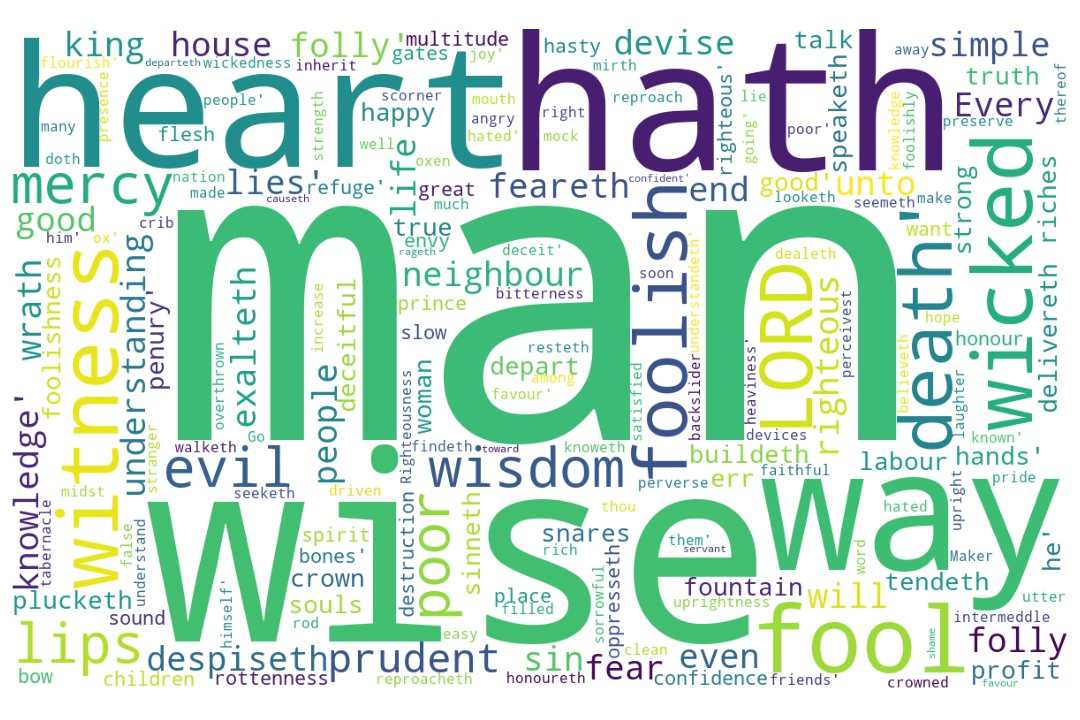
\includegraphics[width=\linewidth]{20OT-Proverbs/Proverb14-WordCloud.jpg}
  \caption{Proverb 14 Word Cloud}
  \label{fig:Proverb 14 Word Cloud}
\end{figure}

\marginpar{\scriptsize \centering \fcolorbox{bone}{lime}{\textbf{WHAT A FOOL DOES}}\\ (Proverbs 14:1-35) \begin{compactenum}[I.][8]
    \item \textbf{Derides Righteousness} (Proverbs 14:9 --  verse with 13 words) \index[scripture]{Proverbs!Pro 14:09}(Pro 14:9)
    \item \textbf{Dealeth in Anger} \index[scripture]{Proverbs!Pro 14:17}(Pro 14:17)
    \item \textbf{Despises Good} \index[scripture]{Proverbs!Pro 14:01, 21}(Pro 14:1, 21)
    \item \textbf{Devises Evil} \index[scripture]{Proverbs!Pro 14:22}(Pro 14:22)
    \item \textbf{Deceives Souls} \index[scripture]{Proverbs!Pro 14:25}(Pro 14:25)
    \item \textbf{Destroys Order} \index[scripture]{Proverbs!Pro 14:28}(Pro 14:28)
    \item \textbf{Deserves Destruction} \index[scripture]{Proverbs!Pro 14:35}(Pro 14:35)
\end{compactenum}}

\marginpar{\scriptsize \centering \fcolorbox{bone}{yellow}{\textbf{7 KINDS OF MEN}}\\ (Proverbs 14:1-35) \begin{compactenum}[I.][8]
    \item The \textbf{False} Man \index[scripture]{Proverbs!Pro 14:05}(Pro 14:5)
    \item The \textbf{Faithful} Man \index[scripture]{Proverbs!Pro 14:05}(Pro 14:5)
    \item The \textbf{Foolish} Man \index[scripture]{Proverbs!Pro 14:08} \index[scripture]{Proverbs!Pro 14:09}  \index[scripture]{Proverbs!Pro 14:24} \index[scripture]{Proverbs!Pro 14:33} (Pro 14:8, 9, 24, 33)
    \item The \textbf{Flourishing} Man \index[scripture]{Proverbs!Pro 14:11} \index[scripture]{Proverbs!Pro 14:35} (Pro 14:11, 35)
    \item The \textbf{Fearing} Man \index[scripture]{Proverbs!Pro 14:16} \index[scripture]{Proverbs!Pro 14:27} (Pro 14:16, 27)
    \item The \textbf{Fleshly} Man \index[scripture]{Proverbs!Pro 14:30} (Pro 14:30)
    \item The \textbf{Favoured} Man \index[scripture]{Proverbs!Pro 14:35} (Pro 14:35)
\end{compactenum}}

\footnote{\textcolor[cmyk]{0.99998,1,0,0}{\hyperlink{TOC}{Return to end of Table of Contents.}}}\footnote{\href{https://audiobible.com/bible/proverbs_14.html}{\textcolor[cmyk]{0.99998,1,0,0}{Proverbs Audio}}}\textcolor[cmyk]{0.99998,1,0,0}{Every wise woman buildeth her house: but the \fcolorbox{bone}{lime}{foolish plucketh it down} with her hands.}
[2] \textcolor[cmyk]{0.99998,1,0,0}{He that walketh in his uprightness feareth the LORD: but \emph{he} \emph{that} \emph{is} perverse in his ways despiseth him.}
[3] \textcolor[cmyk]{0.99998,1,0,0}{In the mouth of the foolish \emph{is} a rod of pride: but the lips of the wise shall preserve them.}
[4] \textcolor[cmyk]{0.99998,1,0,0}{Where no oxen \emph{are}, the crib \emph{is} clean: but much increase \emph{is} by the strength of the ox.}
[5] \textcolor[cmyk]{0.99998,1,0,0}{A faithful witness will not lie: but a false witness will utter lies.}
[6] \textcolor[cmyk]{0.99998,1,0,0}{A scorner seeketh wisdom, and \emph{findeth} \emph{it} not: but knowledge \emph{is} easy unto him that \fcolorbox{bone}{MYGOLD}{understandeth}.}
[7] \textcolor[cmyk]{0.99998,1,0,0}{Go from the presence of a foolish man, when thou perceivest not \emph{in} \emph{him} the lips of knowledge.}
[8] \textcolor[cmyk]{0.99998,1,0,0}{The wisdom of the prudent \emph{is} to understand his way: but the folly of fools \emph{is} deceit.}
[9] \textcolor[cmyk]{0.99998,1,0,0}{Fools make a \fcolorbox{bone}{lime}{mock at sin}: but among the righteous \emph{there} \emph{is} favour.}
[10] \textcolor[cmyk]{0.99998,1,0,0}{The heart knoweth his own bitterness; and a stranger doth not intermeddle with his joy.}
[11] \textcolor[cmyk]{0.99998,1,0,0}{The house of the wicked shall be overthrown: but the tabernacle of the upright shall flourish.}
[12] \textcolor[cmyk]{0.99998,1,0,0}{There is a way which seemeth right unto a man, but the end thereof \emph{are} the ways of death.}\footnote{\textbf{Deuteronomy 12:8} - Ye shall not do after all the things that we do here this day, every man whatsoever is right in his own eyes.}\footnote{\textbf{Judges 17:6} - In those days \emph{there} \emph{was} no king in Israel, \emph{but} every man did \emph{that} \emph{which} \emph{was} right in his own eyes.}\footnote{\textbf{Judges 21:25} - In those days \emph{there} \emph{was} no king in Israel: every man did \emph{that} \emph{which} \emph{was} right in his own eyes.}\footnote{\textbf{Proverb 21:2} - Every way of a man is right in his own eyes: but the LORD pondereth the hearts.}
[13] \textcolor[cmyk]{0.99998,1,0,0}{Even in laughter the heart is sorrowful; and the end of that mirth \emph{is} heaviness.}
[14] \textcolor[cmyk]{0.99998,1,0,0}{The backslider in heart shall be filled with his own ways: and a good man \emph{shall} \emph{be} \emph{satisfied} from himself.}
[15] \textcolor[cmyk]{0.99998,1,0,0}{The simple believeth every word: but the prudent \emph{man} looketh well to his going.}
[16] \textcolor[cmyk]{0.99998,1,0,0}{A wise \emph{man} feareth, and departeth from evil: but the fool rageth, and is confident.}
[17] \textcolor[cmyk]{0.99998,1,0,0}{\emph{He} \emph{that} \emph{is} \fcolorbox{bone}{lime}{soon angry} dealeth foolishly: and a man of wicked devices is hated.}
[18] \textcolor[cmyk]{0.99998,1,0,0}{The simple inherit folly: but the prudent are crowned with knowledge.}
[19] \textcolor[cmyk]{0.99998,1,0,0}{The evil bow before the good; and the wicked at the gates of the righteous.}
[20] \textcolor[cmyk]{0.99998,1,0,0}{The poor is hated even of his own neighbour: but the rich \emph{hath} many friends.}
[21] \textcolor[cmyk]{0.99998,1,0,0}{He that \fcolorbox{bone}{lime}{despiseth his neighbour} sinneth: but he that hath mercy on the poor, happy \emph{is} he.}
[22] \textcolor[cmyk]{0.99998,1,0,0}{Do they not err that \fcolorbox{bone}{lime}{devise evil}? but mercy and truth \emph{shall} \emph{be} to them that devise good.}
[23] \textcolor[cmyk]{0.99998,1,0,0}{In all labour there is profit: but the talk of the lips \emph{tendeth} only to penury.}
[24] \textcolor[cmyk]{0.99998,1,0,0}{The crown of the wise \emph{is} their riches: \emph{but} the foolishness of fools \emph{is} folly.}
[25] \textcolor[cmyk]{0.99998,1,0,0}{A true witness delivereth souls: but a \fcolorbox{bone}{lime}{deceitful \emph{witness}} speaketh lies.}
[26] \textcolor[cmyk]{0.99998,1,0,0}{In the fear of the LORD \emph{is} strong confidence: and his children shall have a place of refuge.}
[27] \textcolor[cmyk]{0.99998,1,0,0}{The fear of the LORD \emph{is} a fountain of life, to depart from the snares of death.}
[28] \textcolor[cmyk]{0.99998,1,0,0}{In the multitude of people \emph{is} the king's honour: but in the want of people \emph{is} the \fcolorbox{bone}{lime}{destruction of the prince}.}
[29] \textcolor[cmyk]{0.99998,1,0,0}{\emph{He} \emph{that} \emph{is} slow to wrath \emph{is} of great \fcolorbox{bone}{MYGOLD}{understanding}: but \emph{he} \emph{that} \emph{is} hasty of spirit exalteth folly.}
[30] \textcolor[cmyk]{0.99998,1,0,0}{A sound heart \emph{is} the life of the flesh: but envy the rottenness of the bones.}
[31] \textcolor[cmyk]{0.99998,1,0,0}{He that oppresseth the poor reproacheth his Maker: but he that honoureth him hath mercy on the poor.}
[32] \textcolor[cmyk]{0.99998,1,0,0}{The wicked is driven away in his wickedness: but the righteous hath hope in his death.}
[33] \textcolor[cmyk]{0.99998,1,0,0}{Wisdom resteth in the heart of him that hath \fcolorbox{bone}{MYGOLD}{understanding}: but \emph{that} \emph{which} \emph{is} in the midst of fools is made known.}
[34] \textcolor[cmyk]{0.99998,1,0,0}{\fcolorbox{bone}{MYGOLD}{Righteousness} exalteth a nation: but sin \emph{is} a reproach to any people.}
[35] \textcolor[cmyk]{0.99998,1,0,0}{The king's favour \emph{is} toward a wise servant: but his \fcolorbox{bone}{lime}{wrath is \emph{against}} him that causeth shame.}


